\chapter{Introduction}

The steady advancement of technology
has automated an increasing variety of menial or dangerous tasks
previously performed by humans.
Computer algorithms now trade our stocks,
route our telephone calls and packages,
and fly our planes,
and simple machines clean our clothes and wash our dishes.

More complex tasks require complex robots with many
degrees of freedom.
Manipulation tasks, in particular,
present challenges in many areas including
perception, symbolic reasoning, and motion planning.
Successful applications have so far been largely
confined to large-scale manufacturing domains,
whose prescribed and structured environments
allow these challenges to be overcome.

However,
manipulation tasks such as clearing a kitchen table
or moving debris in a dangerous disaster scenario
can not yet be planned for quickly and reliably.
\begin{quote}
\emph{%
This thesis proposes an
efficient and robust motion planning approach
well-suited
to articulated robots
performing recurring manipulation tasks
in dynamic, unstructured environments.
}
\end{quote}

We outline the general structure of multi-step manipulation planning
in Chapter~\ref{chap:formulation}.
There are two principal challenges inherent in
human-scale manipulation tasks
that must be addressed by such approaches,
which we review here.

\textbf{Challenge 1: Task Efficiency.}

Autonomous systems performing manipulation tasks are
resource-constrained.
If a home robot takes thirty minutes to clear a table,
or a disaster response robot exhausts its battery ten minutes
into its mission,
these robots will not see widespread use.
These metrics are only meaningful
when applied across the entire task,
from the point it is assigned to the robot
to the point it is complete.

In order to accomplish such a manipulation task,
an autonomous robot must expend two types of effort.
First, it must allocate computation to \emph{plan}
a sequence of motions that will acheive the task.
Second, it must \emph{execute} these plans using its actuators.
Generally, there is a tradeoff between these two;
spending more effort during planning produces paths that are
cheaper to execute.
Planning costs are dominated by \emph{validity checking} --
e.g. checking whether configurations are free from collision.

Robots performing real-world human-scale manipulation tasks
tend to expend comparable effort in these two areas
(see Figure~\ref{fig:plan-exec-cost}).
While some approaches (e.g. anytime planning) attempt to capture
this tradeoff,
our approach,
the Greedy PRM (Chapter~\ref{chap:inflate}),
instead explicitly optimizes for both planning
and execution effort
given a planning effort model.
This allows the planner to determine the proper allocation of effort
between planning and execution in order to minimize total task cost.

Next, Chapter~\ref{chap:graphs-in-continuous}
discusses how to embed these roadmaps efficiently
into continuous configuration spaces,
touching on completeness,
efficiency, etc.

{
\setlength{\offsetpage}{0.5in}
\begin{figure}
\begin{widepage}
\begin{center}
   \begin{subfigure}[b]{1.4in}
      \begin{center}
      \includegraphics{build/intro-cost-herb}
      \end{center}
      \caption{\textsc{Herb} Home Robot}
   \end{subfigure}%
   \quad%
   \begin{subfigure}[b]{2.0in}
      \begin{center}
      \includegraphics{build/intro-cost-chimp}
      \end{center}
      \caption{\textsc{Chimp} Disaster Response Robot}
   \end{subfigure}%
   \quad%
   \begin{subfigure}[b]{2.0in}
      \begin{center}
      \includegraphics{build/intro-cost-axis}
      \end{center}
      \caption{Planning vs. Execution Cost}
   \end{subfigure}
   \caption{For manipulation tasks,
      both the \textsc{Herb} \cite{srinivasa2012herb20}
      and \textsc{Chimp} \cite{stentz2014chimp} robots
      incur comparable cost (e.g. time or energy)
      during planning and execution.
      Our approach considers both explicitly.}
   \label{fig:plan-exec-cost}
\end{center}
\end{widepage}
\end{figure}
}

\textbf{Challenge 2: Sub-Problem Structure.}

While planning cost is a significant component
in resource-constrained human-scale problems,
manipulation tasks exhibit a structure
which makes it difficult to apply fast planning approaches.
In particular,
they are inherently composed of multiple distinct sub-problems,
each of which 
must be validated a different subset of configuration space.
For example, see the manipulation task in
Figure~\ref{fig:intro-multi-step}.

We could do na\"{\i}ve planning, like in the
DRC Trials \cite{dellin2014drc},
with no reuse.
We call a single-query planner for each step.
Either we generate roots at the start,
or we let each sub-planner pick a root it can get to, and commit.
First, we can get stuck,
comitting to something that either is infeasible, or takes too long.
Second, this is too slow --
each sub-plan simply takes too long.

We could try multi-query planning,
but as mentioned,
the valid subset changes for each step.

We solve this in two ways.
First, in Chapter~\ref{chap:multi-set},
we introduce the multi-set planning problem.
We show that while the valid subsets are different for each step,
they are related in a structured way.
In fact, we show how lots of different prior ideas for planner
efficiency are unified by this formalism.

Second, Chapter~\ref{chap:multi-set-prm}
uses the multi-set formalism as a planning cost model
for use by the Greedy PRM.
The resulting algorithm,
the Multi-Set PRM,
uses propositional logic to represent multi-set stuff
algorithmically.
We show how we can incremental graph search approaches
to make it super fast.

{
\setlength{\offsetpage}{0.75in}
\begin{figure}
\begin{widepage}
\begin{center}

\begin{subfigure}[t]{0.19\linewidth}
\centering
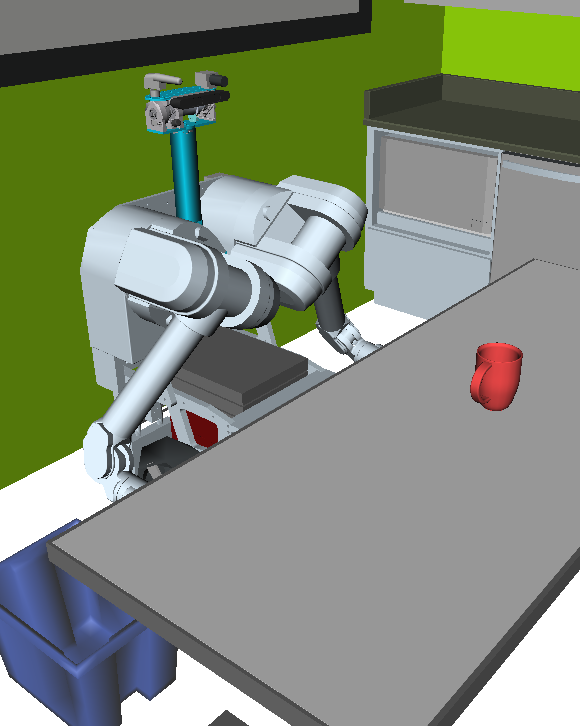
\includegraphics[width=\columnwidth]{figs/testherb-a.png}
\caption{Start config}
\end{subfigure}
\begin{subfigure}[t]{0.19\linewidth}
\centering
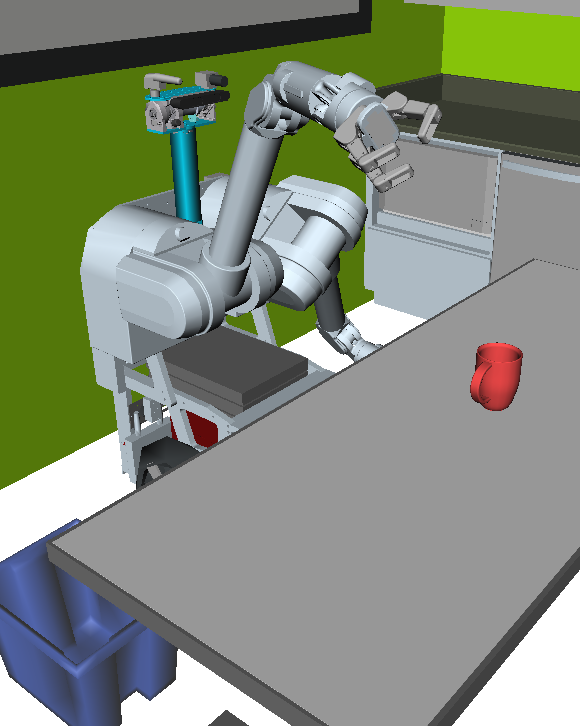
\includegraphics[width=\columnwidth]{figs/testherb-b.png}
\caption{Step 1 in $X_1$}
\end{subfigure}
\begin{subfigure}[t]{0.19\linewidth}
\centering
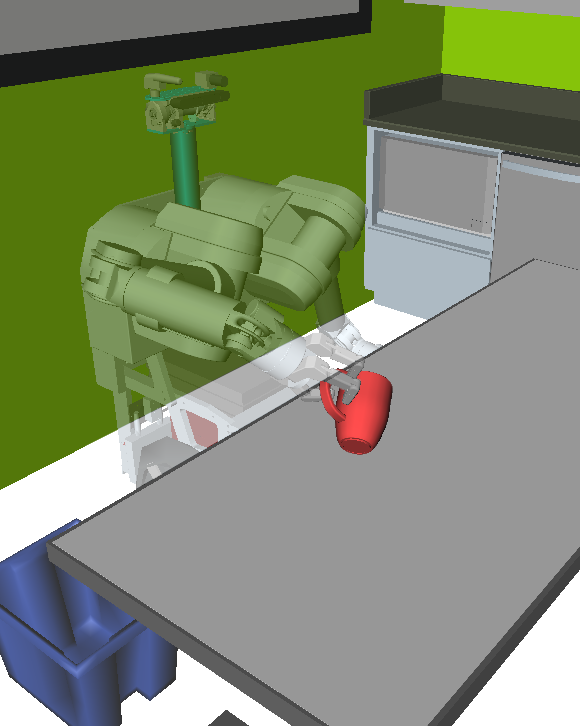
\includegraphics[width=\columnwidth]{figs/testherb-c.png}
\caption{Step 2 in $X_2$}
\end{subfigure}
\begin{subfigure}[t]{0.19\linewidth}
\centering
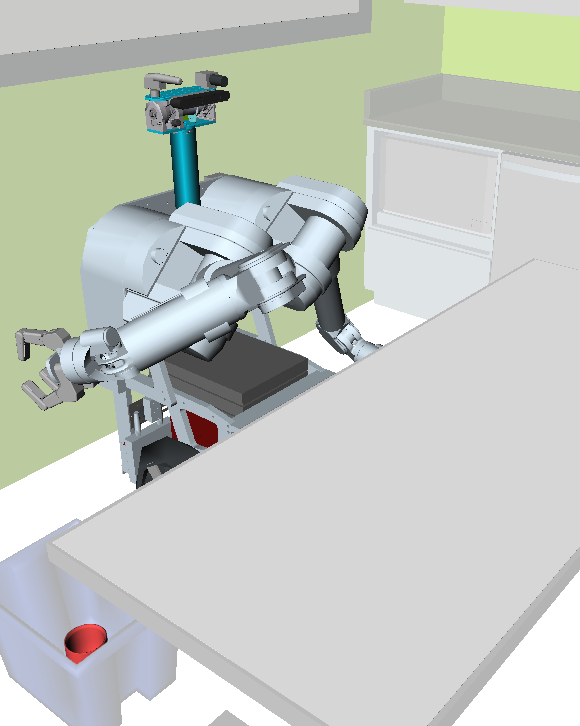
\includegraphics[width=\columnwidth]{figs/testherb-d.png}
\caption{Step 3 in $X_3$}
\end{subfigure}
\begin{subfigure}[t]{0.19\linewidth}
\centering
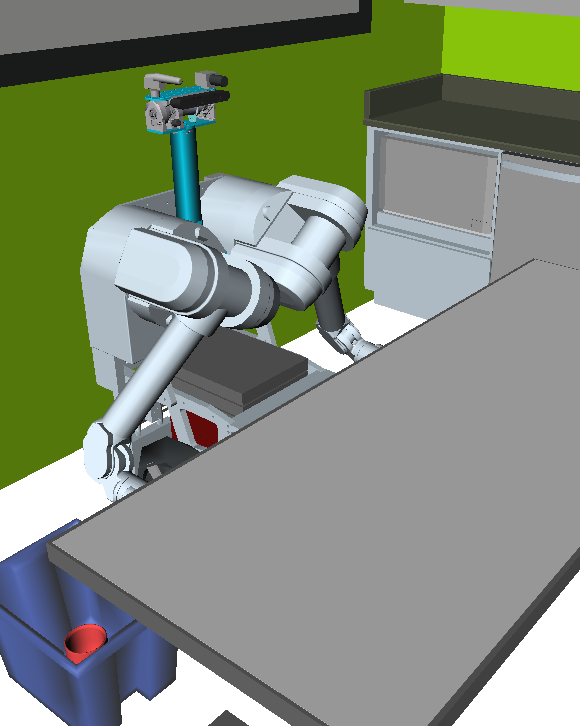
\includegraphics[width=\columnwidth]{figs/testherb-e.png}
\caption{End config}
\end{subfigure}

\vspace{0.1in}

   \begin{subfigure}[b]{4.0in}
      \begin{center}
      \includegraphics{build/intro-subprob-cspace}
      \end{center}
      \caption{Plan sequences
         within distinct free $\mathcal{C}$-subsets
         from the problem above.}
   \end{subfigure}%
   \quad%
   \begin{subfigure}[b]{2.0in}
      \begin{center}
      \includegraphics{build/intro-subprob-axis}
      \end{center}
      \caption{Single vs. Multi Query Planners}
   \end{subfigure}
   \caption{\textsc{Herb} plans for a simple manipulation task
      to grasp, transfer, and drop a mug from a table into a bin
      before returning to an end configuration.
      Each sub-problem requires a path in a distinct free subset of
      configuration space;
      our approach enables partial reuse between these steps.}
   \label{fig:intro-multi-step}
\end{center}
\end{widepage}
\end{figure}
}

\textbf{Applications and Experiments}

We give a bunch of examples of this framework
for different robots.
For example, I really want to talk about robots idly
hypothesizing worlds.

{
\setlength{\offsetpage}{0.75in}
\begin{figure}
\begin{widepage}
\begin{center}
\begin{tikzpicture}

% axes
\draw[->,thick] (0,0) -- (0,8); 
\draw[->,thick] (0,0) -- (12,0);
\node[rotate=90,align=center] at (-1.0,4)
   {Challenge 1:\\Task Efficiency};
\node[align=center] at (6,-1.6)
   {Challenge 2:\\Sub-Problem Structure};

% y tics
\draw (-0.2,1) -- (0.2,1);
\node[rotate=90,align=center] at (-0.64,1)
   {considers\\[-0.04in]execution cost};
\draw (-0.2,7) -- (0.2,7);
\node[rotate=90,align=center] at (-0.8,7)
   {considers\\[-0.04in]planning and\\[-0.04in]execution cost};

% x tics
\draw (2,-0.2) -- (2,0.2);
\node[align=center] at (2,-0.5) {no reuse};
\draw (6,-0.2) -- (6,0.2);
\node[align=center] at (6,-0.5) {two-set reuse};
\draw (10,-0.2) -- (10,0.2);
\node[align=center] at (10,-0.5) {full reuse};

% algorithms
\node[draw,ellipse,align=center] at (2,1)
   {Lazy PRM \cite{bohlin2000lazyprm}};

\node[draw,ellipse,align=center] at (6,1)
   {\cite{leven2000changing}, \cite{kallman2004dynamicroadmaps},
   \cite{jaillet2004dynamicprm}};

\node[draw,ellipse,align=center] at (2,7)
   {Greedy PRM\\(Chapter~\ref{chap:inflate})};

\node[draw,ellipse,align=center] at (10,7)
   {Multi-Set PRM\\(Chapter~\ref{chap:multi-set-prm})};

\end{tikzpicture}
\caption{Graphical outline of $\mathcal{C}$-space planners.
   Work in progress.}
\label{fig:graphical-outline}
\end{center}
\end{widepage}
\end{figure}
}
